\documentclass[12]{report}

\usepackage{amssymb,amsmath}

%\usepackage{refcheck}

\usepackage{graphicx}
\usepackage{amssymb}
\usepackage{mathrsfs}
\usepackage{amsmath}
\usepackage{latexsym}
\usepackage{amssymb}
\usepackage{enumerate}
\usepackage{fullpage} 
\usepackage{setspace}
\usepackage{color}
%\usepackage{ dsfont }
\usepackage{float}
\usepackage{physics}
\usepackage{hyperref}

%new math symbols taking no arguments
\newcommand\0{\mathbf{0}}
\newcommand\CC{\mathbb{C}}
\newcommand\FF{\mathbb{F}}
\newcommand\NN{\mathbb{N}}
\newcommand\QQ{\mathbb{Q}}
\newcommand\RR{\mathbb{R}}
\newcommand\ZZ{\mathbb{Z}}
\newcommand\bb{\mathbf{b}}
\newcommand\kk{\Bbbk}
\newcommand\mm{\mathfrak{m}}
\newcommand\pp{\mathfrak{p}}
\newcommand\xx{\mathbf{x}}
\newcommand\yy{\mathbf{y}}
\newcommand\GL{\mathit{GL}}
\newcommand\into{\hookrightarrow}
\newcommand\nsub{\trianglelefteq}
\newcommand\onto{\twoheadrightarrow}
\newcommand\minus{\smallsetminus}
\newcommand\goesto{\rightsquigarrow}
\newcommand\nsubneq{\vartriangleleft}

%redefined math symbols taking no arguments
\newcommand\<{\langle}
\renewcommand\>{\rangle}
\renewcommand\iff{\Leftrightarrow}
\renewcommand\phi{\varphi}
\renewcommand\implies{\Rightarrow}

%new math symbols taking arguments
\newcommand\ol[1]{{\overline{#1}}}

%redefined math symbols taking arguments
\renewcommand\mod[1]{\ (\mathrm{mod}\ #1)}

%roman font math operators
\DeclareMathOperator\aut{Aut}

%for easy 2 x 2 matrices
\newcommand\twobytwo[1]{\left[\begin{array}{@{}cc@{}}#1\end{array}\right]}

%for easy column vectors of size 2
\newcommand\tworow[1]{\left[\begin{array}{@{}c@{}}#1\end{array}\right]}

\newtheorem{theorem}{Theorem}[section]
\newtheorem{corollary}{Corollary}[theorem]
\newtheorem{lemma}[theorem]{Lemma}
\newtheorem{exercise}[theorem]{Exercise}
\newtheorem{definition}[theorem]{Definition}

\title{PHY 781: Final Project}
\author{Faris Sbahi}

\begin{document}
\maketitle

\chapter{Project 1}

Define the lattice action

\begin{align*}
S^l_E = \sum_x \{ \frac{1}{2} \chi_x^2 - \frac{\kappa}{2} \sum_{\mu} \chi_x \chi_{x + \hat{\mu}} + g \chi_x^4 \}
\end{align*}

\begin{align*}
\kappa^{-1} := 2d + \alpha \\
\alpha := (m_0a)^2
\end{align*}

\begin{align*}
\sigma &= \frac{1}{L^d}\sum_x \langle \chi^2_x \rangle\\
\chi &= \frac{1}{L^d}\sum_{x,y} \langle \chi_x \chi_y \rangle\\
F &= \frac{1}{L^d}\sum_{x,y} \langle \chi_x \chi_y \rangle \cos (2 \pi \Delta \tau / L)
\end{align*}

and furthermore

\begin{align*}
M(L) &= 	\frac{2 \sin (\pi / L)}{\sqrt{(\chi / F) - 1}}
\end{align*}


By definition,

\begin{align*}
\langle \phi(x) \phi(y)\rangle = \frac{1}{Z} \int [d \phi] e^{-S_E(\phi)} \phi(x) \phi(y)
\end{align*}

where 


\begin{align*}
Z = \int [d\phi] e^{-S_E(\phi)}
\end{align*}

\section{Exact Computation}

\subsection{$g=0$ and $\kappa \neq 0$}

We can construct $S$ as a matrix-vector product in terms of $M$

\begin{align*}
S_E^l &= \frac{1}{2}\chi_{i}M_{ij}\chi_{j}\\
M_{ij} &= - \kappa \sum_{\mu} (\delta_{i + \mu, j} + \delta_{i - \mu, j}) + \delta_{ij}
\end{align*}

where $i + \mu$ translates $i$ to all forward neighbors in $d$ dimensions i.e. $\mu = (0, \cdots , a, \cdots 0)$. Hence, $\sum_y M(x - y)M^{-1}(y-z) = \delta_{x,z}$ implies that 

\begin{align*}
\sum_y [- \kappa \sum_{\mu} (\delta_{x + \mu, y} + \delta_{x - \mu, y}) + \delta_{xy}] M^{-1}(y-z) = \delta_{x,z}
\end{align*}

In momentum space, we have

\begin{align*}
\sum_y [- \kappa \sum_{\mu} (\delta_{x + \mu, y} + \delta_{x - \mu, y}) + \delta_{xy}] M^{-1}(y-z) &\rightarrow \sum_y \int_{- \pi / a}^{\pi / a} \frac{d^d k}{(2\pi)^d} e^{ik \cdot (y - z)} \tilde{M}^{-1}(k) [- \kappa \sum_{\mu} (\delta_{x + \mu, y} + \delta_{x - \mu, y}) + \delta_{xy}]  \\
&= \int_{- \pi / a}^{\pi / a} \frac{d^d k}{(2\pi)^d} \tilde{M}^{-1}(k) [- \kappa \sum_{\mu} (e^{ik \cdot (x + \mu - z)} + e^{ik \cdot (x - \mu - z)}) + e^{ik \cdot (x - z)}] \\
&= \int_{- \pi / a}^{\pi / a} \frac{d^d k}{(2\pi)^d} \tilde{M}^{-1}(k) [- \kappa \sum_{\mu} (e^{ik \cdot \mu} + e^{-ik \cdot \mu}) + 1]e^{ik \cdot (x - z)} \\
\delta_{x,z} &\rightarrow \int_{- \pi / a}^{\pi / a} \frac{d^d k}{(2\pi)^d} e^{ik \cdot (x - z)}
\end{align*}

Therefore, we can conclude that 

\begin{align*}
	\tilde{M}^{-1}(k) [- \kappa \sum_{\mu} (e^{ik \cdot \mu} + e^{-ik \cdot \mu}) + 1] &= 1 \\
	\tilde{M}^{-1}(k) &= \frac{1}{1 - \kappa \sum_{\mu} (e^{ik \cdot \mu} + e^{-ik \cdot \mu})} \\
	&= \frac{1}{1 - 2\kappa \sum_{\mu} \cos(k \cdot \mu)}
\end{align*}

So, we can write that the momentum in the $\mu$ direction as $k_\mu := k \cdot \mu$. Note that momentum is restricted to the Brillouin zone: $|k_\mu| \leq \pi$. Because the lattice is discretized and each dimension is of size $L$, $k_\mu$ takes on values

\begin{align*}
	k_\mu = \frac{2\pi n_\mu}{L}, \qquad n_\mu \in \{0, \cdots, L - 1 \}
\end{align*}

which gives

\begin{align*}
	\tilde{M}^{-1}(k) &= \frac{1}{1 - 2\kappa \sum_{\mu} \cos(\frac{2\pi n_\mu}{L})}
\end{align*}


Now, note that

\begin{align*}
\sum_x \chi_x^2 &= \sum_x \bra{\chi}\ket{x}	\bra{x}\ket{\chi}\\
&= \sum_k \bra{\chi}\ket{k}	\bra{k}\ket{\chi}\\
\sigma &= \frac{1}{L^d}\sum_k \langle \chi^2_k \rangle\\
&=  \sum_{n_1, \cdots, n_d} \frac{1}{1 - 2\kappa \sum_{\mu} \cos(\frac{2\pi n_\mu}{L})}
\end{align*}

Furthermore, since $|\bra{k=0}\ket{x}|^2 = \frac{e^{0}}{L^d}$ 

\begin{align*}
\sum_{x,y} \chi_x \chi_y &= \frac{1}{L^d} \sum_{x, y} \bra{\chi}\ket{x}  \bra{y}\ket{\chi} \\
&= \sum_{x, y, k, k'} \bra{\chi}\ket{k}\bra{k}\ket{x}\bra{x}\ket{0}\bra{0}\ket{y} \bra{y}\ket{k'}\bra{k'}\ket{\chi} \\
&= |\bra{k=0}\ket{\chi}|^2 \\
\chi &= \langle \chi^2_{k={(0, \cdots, 0)}} \rangle \\
&= \frac{1}{1 - 2\kappa d}
\end{align*}

Finally, using $\cos(2\pi (x_0 - y_0) / L) = (e^{2\pi i (x_0 - y_0) / L} + e^{-2\pi i (x_0 - y_0) / L})/2$ where $x_0$ is the component of $x$ along the time dimension,

\begin{align*}
\sum_{x_0,y_0} \chi_x \chi_y e^{2\pi i (x_0 - y_0) / L} &= \sum_{x_0,y_0}  \bra{\chi}\ket{x_0} \bra{x_0}\ket{k = 1} \bra{k = 1}\ket{y_0} \bra{y_0}\ket{\chi} \\
\intertext{and the same follows for complex conjugate $\sum_{x_0,y_0} \chi_x \chi_y e^{-2\pi i (x_0 - y_0) / L}$. Hence, using this result and $\chi$ above, }
F &= \langle \chi^2_{k={(1, 0, \cdots, 0)}} \rangle  \\
&= \frac{1}{1 - 2\kappa [\cos(\frac{2\pi}{L}) + d-1]}
\end{align*}

Using these derived relations, we find the following results for $L = 16, g = 0, \alpha = 0.25$,

\begin{table}[H]
\label{table:exact-kappa}
\centering
\begin{tabular}{|l|l|l|l|l|}
\hline
$d$ & $\sigma$          & $\chi$             & $F$                & $M(L)$ \\ \hline
2   & 1.6021 & 17.0000 & 10.5659 & 0.5000    \\
3   & 1.3198 & 25.0000  & 15.5380 &   0.5000  \\
4   & 1.1995  &  33.0000  & 20.5101  &    0.5000 \\ \hline
\end{tabular}
\caption{Exact Computation Results for $g=0$ and $\kappa \neq 0$}
\end{table}

\subsection{$g\neq 0$ and $\kappa = 0$}

\section{Monte Carlo for $g=0$ or $\kappa = 0$}

\subsection{$g=0$ and $\kappa \neq 0$}

We used the Monte Carlo algorithm with 10,000 spin and regular updates. We found the following results for $L = 16, g = 0, \alpha = 0.25$.

\begin{table}[H]
\centering
\begin{tabular}{|l|l|l|l|l|}
\hline
$d$ & $\sigma$ & $\chi$ & $F$ & $M(L)$ \\ \hline
2   & 1.5984 & 16.9759 & 10.5659 & 0.5104 \\
3   & 1.3201 & 24.5100 & 15.3275 & 0.5041 \\
4   & 1.1995  &  32.8455 & 20.3969  & 0.4994 \\ \hline
\end{tabular}
\caption{Monte Carlo Results for $g=0$ and $\kappa \neq 0$}
\end{table}

which aligns closely with Table \ref{table:exact-kappa}

\subsection{$g\neq 0$ and $\kappa = 0$}

We used the Monte Carlo algorithm with 10,000 spin and regular updates. We found the following results for $L = 16, g = 0.1, \kappa = 0, \alpha = 0.25$.

\begin{table}[H]
\centering
\begin{tabular}{|l|l|l|l|l|}
\hline
$d$ & $\sigma$ & $\chi$ & $F$ & $M(L)$ \\ \hline
2   & 0.6150 & 0.6151 & 0.6151 & $\infty$ \\
3   & 0.6156 & 0.6241 & 0.6241 & $\infty$  \\
4   & 0.6155  & 0.6211 & 0.6211  & $\infty$ \\ \hline
\end{tabular}
\caption{Monte Carlo Results for $g\neq 0$ and $\kappa = 0$}
\end{table}

which aligns closely with Table \ref{}

\section{Monte Carlo for $g\neq0$ and $\kappa \neq 0$}

% TODO - add errors

We used the Monte Carlo algorithm with 10,000 spin and regular updates. We found the following results for $L = 8, g = 0.1, \alpha = -1.5$.

\begin{table}[H]
\centering
\begin{tabular}{|l|l|l|l|l|}
\hline
$d$ & $\sigma$ & $\chi$ & $F$ & $M(L)$ \\ \hline
2   & 0.8295 & 6.0336 & 2.4549 & 0.6339 \\
3   & 0.6855 & 2.8406 & 2.0802 & 1.2659  \\
4   & 0.6562  & 2.3761 & 1.9910  & 1.7403 \\ \hline
\end{tabular}
\caption{Monte Carlo Results for $g\neq 0$ and $\kappa = 0$}
\end{table}


\chapter{Project 2}

\section{Computing the Physical Mass}

\section{Computing the Lattice Spacing}

\begin{figure}[H]
\centering
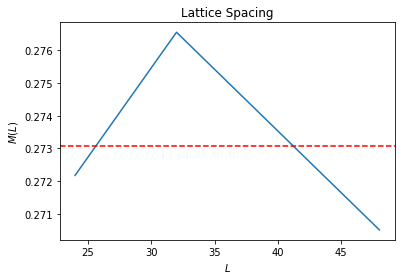
\includegraphics[width=0.7\textwidth]{lattice_spacing.png}
\caption{We see that $M(L)$ approaches a constant near $0.273$ as $L$ increases as seen by plotting $L = 24, 32, 48$.}	
\end{figure}


\section{Renormalization}

\subsection{$d=2$}

\begin{figure}[H]
\centering
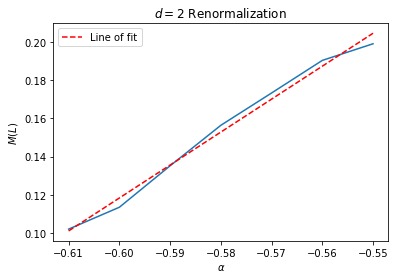
\includegraphics[width=0.7\textwidth]{renormalization_2}
\caption{$M_{phys}a$ can be given in terms of the tuning parameter roughly by $1.724(\alpha + 0.669)$}	
\end{figure}


\subsection{$d=3$}

\begin{figure}[H]
\centering
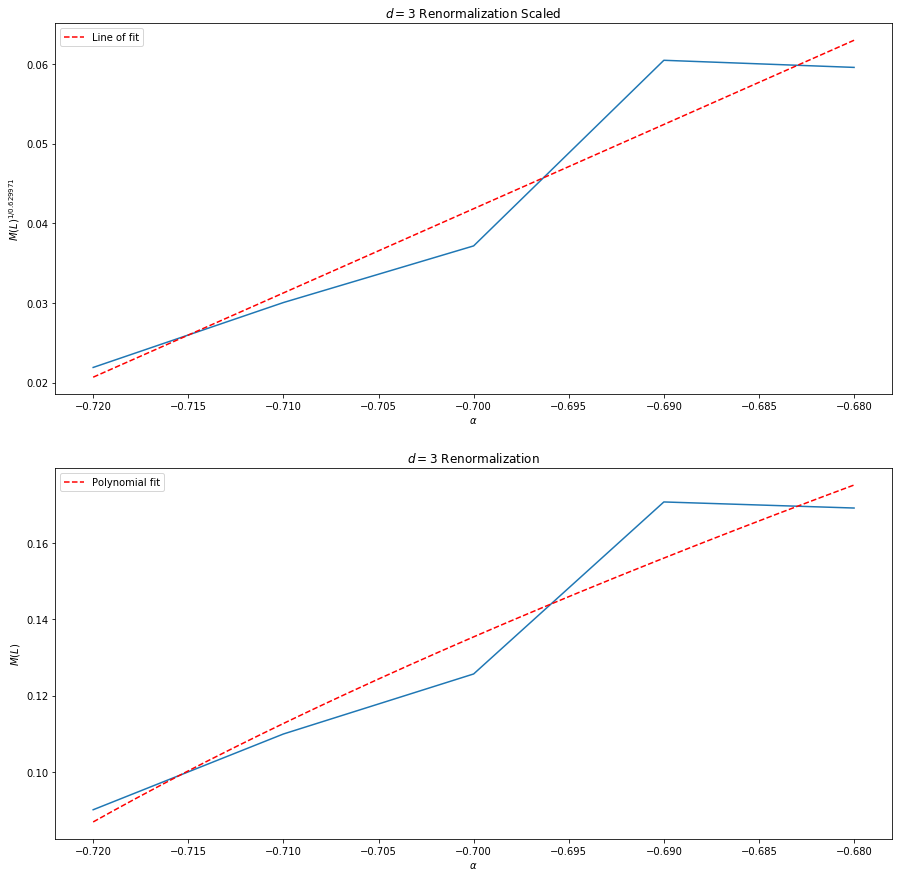
\includegraphics[width=\textwidth]{renormalization_3}
\caption{$M_{phys}a$ can be given in terms of the tuning parameter roughly by $1.036(\alpha + 0.740)^{0.629971}$}		
\end{figure}

\subsection{$d=4$}

\begin{figure}[H]
\centering
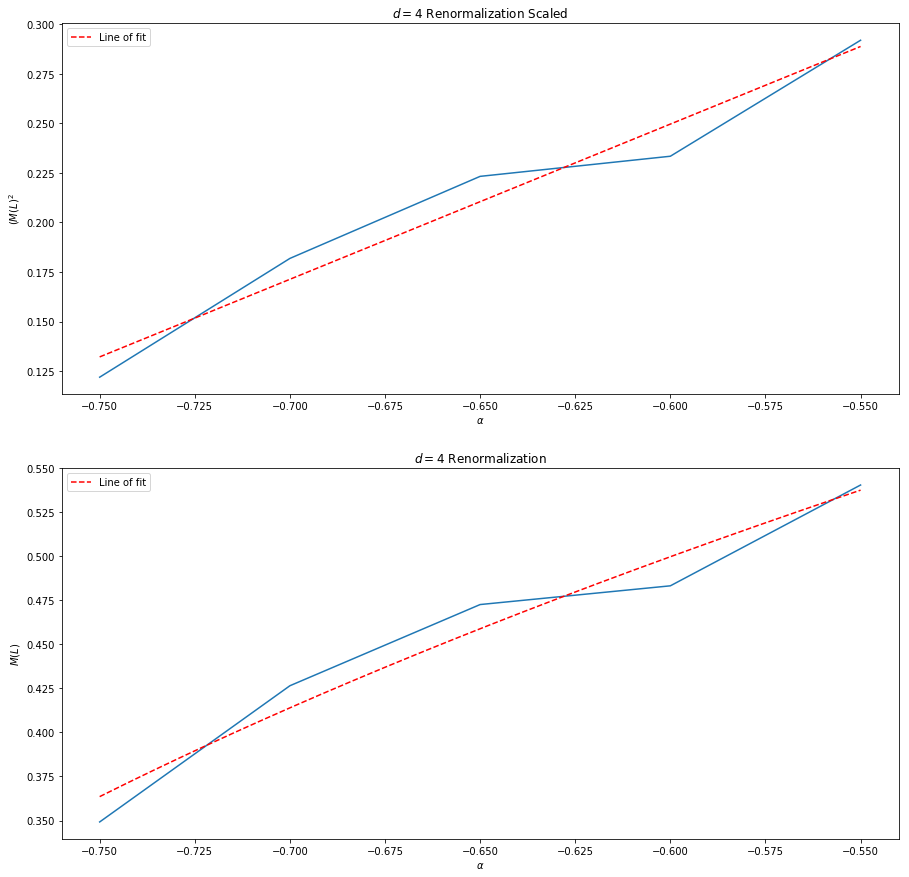
\includegraphics[width=\textwidth]{renormalization_4}
\caption{$M_{phys}a$ can be given in terms of the tuning parameter roughly by $0.885(\alpha + 0.919)^{0.5}$}		
\end{figure}

\section{Spontaneous Symmetry Breaking}


\end{document}
